\documentclass{standalone}
\usepackage{tikz}
\usetikzlibrary{shapes,arrows,positioning,fit,backgrounds}

\begin{document}
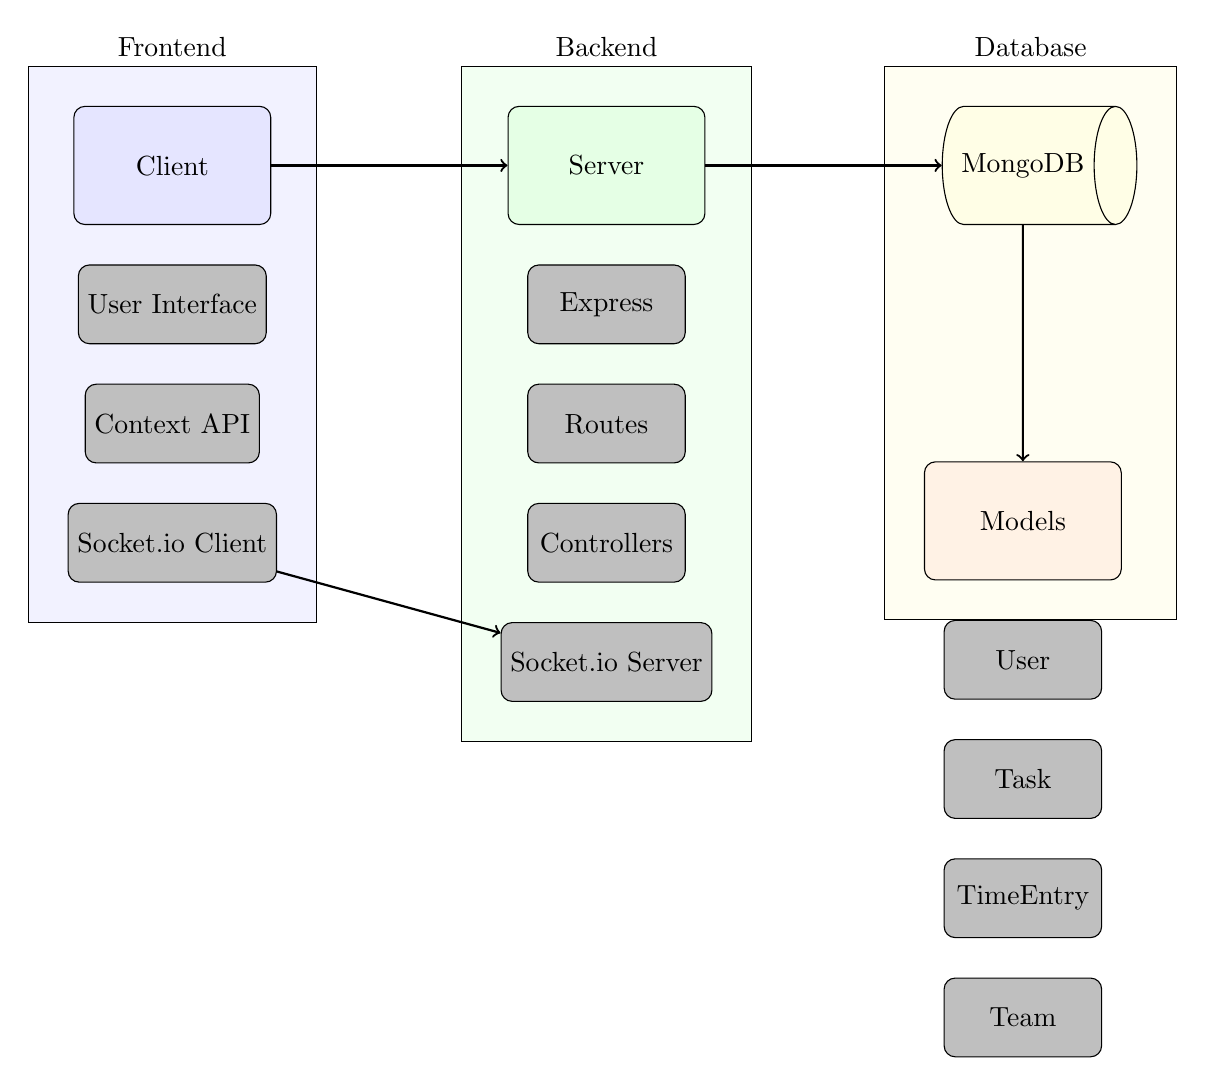
\begin{tikzpicture}[
    node distance=1.5cm,
    box/.style={rectangle, draw, minimum width=2.5cm, minimum height=1.5cm, text centered, rounded corners},
    arrow/.style={->, thick},
    cloud/.style={cloud, draw, minimum width=2.5cm, minimum height=1.5cm, text centered},
    database/.style={cylinder, draw, minimum width=1.5cm, minimum height=2cm, text centered},
    component/.style={rectangle, draw, minimum width=2cm, minimum height=1cm, text centered, rounded corners, fill=lightgray}
]

% Client-side components
\node[box, fill=blue!10] (client) {Client};
\node[component, below=0.5cm of client] (ui) {User Interface};
\node[component, below=0.5cm of ui] (context) {Context API};
\node[component, below=0.5cm of context] (socket-client) {Socket.io Client};

% Server-side components
\node[box, fill=green!10, right=3cm of client] (server) {Server};
\node[component, below=0.5cm of server] (express) {Express};
\node[component, below=0.5cm of express] (routes) {Routes};
\node[component, below=0.5cm of routes] (controllers) {Controllers};
\node[component, below=0.5cm of controllers] (socket-server) {Socket.io Server};

% Database
\node[database, fill=yellow!10, right=3cm of server] (db) {MongoDB};

% Models
\node[box, fill=orange!10, below=3cm of db] (models) {Models};
\node[component, below=0.5cm of models] (user-model) {User};
\node[component, below=0.5cm of user-model] (task-model) {Task};
\node[component, below=0.5cm of task-model] (time-model) {TimeEntry};
\node[component, below=0.5cm of time-model] (team-model) {Team};

% Connections
\draw[arrow] (client) -- (server);
\draw[arrow] (server) -- (db);
\draw[arrow] (db) -- (models);
\draw[arrow] (socket-client) -- (socket-server);

% Background
\begin{scope}[on background layer]
    \node[fit=(client)(socket-client), draw, inner sep=0.5cm, fill=blue!5, label=above:Frontend] {};
    \node[fit=(server)(socket-server), draw, inner sep=0.5cm, fill=green!5, label=above:Backend] {};
    \node[fit=(db)(models), draw, inner sep=0.5cm, fill=yellow!5, label=above:Database] {};
\end{scope}

\end{tikzpicture}
\end{document} 